\subsection{Setting and related literature}

We start by introducing in Sections~\ref{subsubsec:discrepancy} and \ref{subsubsec:sbp} two sets of independent definitions and models,
both being important motivations behind the problem we study, which is discussed in Section~\ref{subsubsec:average_mdiscrepancy}.

\subsubsection{Discrepancy theory}\label{subsubsec:discrepancy}

Computing the \emph{discrepancy} (i.e.\ the best possible balancing) of a collection of sets or vectors 
is a classical question in mathematics and theoretical computer science. 
It has wide-ranging applications in combinatorics, computational geometry,
experimental design, and the theory of approximation algorithms, to name a few. 
The reader will find in \cite{spencer1994ten,matousek2009geometric,chen2014panorama} a detailed account of the history and applications of 
discrepancy theory.
Arguably one of the most celebrated results in this area is the following theorem, known as Spencer's ``six deviations suffice''~\citep{spencer1985six}.
\begin{theorem}[\cite{spencer1985six}]
    \label{thm:spencer}
    There exists $C > 0$ such that for all $n, d \geq 1$, and all $\bu_1, \cdots, \bu_n \in \bbR^d$ with $\|\bu_i\|_\infty \leq 1$ for all $i \in [n]$: 
    \begin{equation*}
       \disc(\bu_1, \cdots, \bu_n) \coloneqq \min_{\eps \in \{\pm 1\}^n} \left\|\sum_{i=1}^n \eps_i \bu_i\right\|_\infty \leq
       \begin{dcases}
       C \sqrt{n \max \left(1, \log \frac{d}{n}\right)} &\textrm{ if } n \leq d, \\
       C \sqrt{d} &\textrm{ if } n > d.
       \end{dcases}
    \end{equation*}
\end{theorem}
\noindent
The second case $n > d$ can be deduced from the result for $n = d$ using classical arguments based on iterated rounding, see e.g.~\cite{spencer1994ten}.
Interestingly, Spencer's theorem shows that one can drastically improve over a naive pick of random signings $\eps_1, \cdots, \eps_n \iid \Unif(\{\pm 1\})$. Indeed, 
it is not hard to show that (taking $n = d$ for simplicity) random signings achieve $\left\|\sum_{i=1}^n \eps_i \bu_i\right\|_\infty = \Theta(\sqrt{n \log n})$ for a worst-case choice of $(\bu_i)_{i=1}^n$, 
with high probability as $n \to \infty$. Spencer's theorem thus implies the existence of a signing $\eps \in \{\pm 1\}^n$, 
which depends on the value of the $\bu_i$'s, and whose discrepancy generically improves over the one of random signs by a logarithmic factor.
While the original proof of \cite{spencer1985six} is not constructive, there has been recently a great number of results regarding efficient algorithmic constructions of 
these signings. We will discuss this point further in Section~\ref{subsec:discussion}.

\myskip 
\textbf{Matrix discrepancy --}
In the present work we consider the problem of \emph{matrix discrepancy}. Given a set of $n$ symmetric $d \times d$ matrices $\bA_1, \cdots, \bA_n$, 
we aim to characterize the following discrepancy objective ($\|\bA\|_\op \coloneqq \max_{\|\bx\|_2=1} \|\bA \bx\|_2$ is the spectral, or operator, norm):
\begin{equation}
    \label{eq:def_disc}
    \disc(\bA_1, \cdots, \bA_n) \coloneqq \min_{\eps \in \{\pm 1\}^n} \left\| \sum_{i=1}^n \eps_i \bA_i \right\|_\op.
\end{equation}
As already mentioned, a foundational question in discrepancy is how the discrepancy objective compares to the one achieved by a \emph{random} choice of the 
signings $\eps_i \iid \Unif(\{\pm 1\})$: matrix discrepancy is thus intimately connected to the study of large random matrices.
Matrix discrepancy has also
been shown to have implications in the theory of quantum random access codes~\citep{hopkins2022matrix,bansal2023resolving}, 
in generalizations of the Kadison-Singer problem~\citep{marcus2015interlacing,kyng2020four}, as well as 
graph sparsification~\citep{batson2014twice} to name a few.

\myskip
The celebrated ``Matrix Spencer'' conjecture~\citep{zouzias2012matrix,meka2014discrepancy1} is likely the most important open problem in matrix discrepancy.
It asserts that Spencer's Theorem~\ref{thm:spencer} can be generalized to the matrix setting, as follows.
\begin{conjecture}[Matrix Spencer~\citep{zouzias2012matrix,meka2014discrepancy1}]\label{conj:mspencer}
    There exists $C > 0$ such that for all $n, d \geq 1$, and all $\bA_1, \cdots, \bA_n$ symmetric $d \times d$ matrices with $\max_{i \in [n]}\|\bA_i\|_\op \leq 1$:
    \begin{equation*}
        \disc(\bA_1, \cdots, \bA_n) \leq C \sqrt{n \max\left(1, \log \frac{d}{n}\right)}.
    \end{equation*}
    In particular, the discrepancy is $\mcO(\sqrt{n})$ for $d = n$.
\end{conjecture}
\noindent
We stress that Spencer's theorem can be seen as the special case of Conjecture~\ref{conj:mspencer} in which all $\bA_i$ commute with each other (and are thus diagonalizable in the same basis).
Moreover, a weaker form of Conjecture~\ref{conj:mspencer}, with a bound $\mcO(\sqrt{n \log d})$ on the right-hand side, can easily be shown to be achievable using a random choice 
of signs $\eps_i \iid \Unif(\{\pm 1\})$, using the non-commutative Khintchine inequality of~\cite{lust1991non}.
Despite a recent surge in efforts~\citep{levy2017deterministic,hopkins2022matrix,dadush2022new}, Conjecture~\ref{conj:mspencer} remains open at the time of this writing. 
The best-known result is a proof of Matrix Spencer if we additionally assume
$\rk(\bA_i) \lesssim n / \log^3 n$~\citep{bansal2023resolving}, and is based on the recent improvements over the non-commutative Khintchine inequality of \cite{bandeira2023matrix}.
In this work, we consider an average-case version of Conjecture~\ref{conj:mspencer}, introduced in Section~\ref{subsubsec:average_mdiscrepancy}.

\subsubsection{Random vector discrepancy, and the symmetric binary perceptron}\label{subsubsec:sbp}

\noindent
A natural question in vector discrepancy (i.e.\ in the setting of Theorem~\ref{thm:spencer}) is to shift our attention to average-case settings, where the $\bu_i$ are 
chosen randomly rather than potentially adversarially.
The typical discrepancy for random vectors is now well understood: in the regime $n = \omega(d)$ (i.e.\ $d = \smallO(n)$, many more signs than dimensions), 
\cite{turner2020balancing} established the following result (with partial results preceding in~\cite{karmarkar1986probabilistic,costello2009balancing}):
\begin{theorem}[\cite{turner2020balancing}]\label{thm:rvector_disc}
    Assume that $\bu_1, \cdots, \bu_n \iid \mcN(0, \Id_d)$ and that $n = \omega(d)$.
    Then  
    \begin{align*}
        \plim_{d \to \infty} \frac{\disc(\bu_1, \cdots, \bu_n)}{\sqrt{\frac{\pi n}{2}} 2^{-n/d}} = 1,
    \end{align*}
    where the limit is meant in probability.
\end{theorem}
\noindent
While Spencer's Theorem~\ref{thm:spencer} does not apply to such random vectors (as one can easily show that $\|\bu_i\|_\infty \sim \sqrt{2 \log d} \gg 1$),
the randomness makes the problem amenable to a detailed mathematical analysis with different tools.

\myskip
In a complementary way, 
recent works have characterized
very precisely the minimal discrepancy in the proportional regime $n = \Theta(d)$, as a function of the ``aspect ratio'' $\beta \coloneqq \lim_{d \to \infty} n/d$.
This setting of random vector discrepancy is an instance of the \emph{symmetric binary perceptron} (SBP), a random constraint satisfaction problem 
which was introduced in~\cite{aubin2019storage}
as a variant to the classical asymmetric binary perceptron. 
The latter is  
a simple model of a neural network storing random patterns, which has a long history of study in 
computer science, statistical physics, and probability theory~\citep{cover1965geometrical,gardner1988space,gardner1988optimal,krauth1989storage,sompolinsky1990learning,talagrand1999intersecting,talagrand2010mean}.
For a \emph{margin} $K > 0$, and in the limit $n/d \to \beta > 0$, the question of satisfiability in the SBP was introduced in~\cite{aubin2019storage} 
as:
\begin{center}
   \textit{
    Given $\bg_1, \cdots, \bg_d \iid \mcN(0, \Id_n)$, can we find $\eps \in \{\pm 1\}^n$ 
    such that $\max_{i \in [d]}|\langle \bg_i, \eps \rangle| \leq K \sqrt{n}$? 
   }
\end{center}
Letting $(\bu_i)_k \coloneqq (\bg_j)_k$, so that $(\bu_i)_{i=1}^n \iid \mcN(0, \Id_d)$ it is clear that the 
the SBP can be thought as an average-case version of vector discrepancy, 
and more precisely to the setting of Theorem~\ref{thm:rvector_disc} with $n = \Theta(d)$.
The SBP has received significant attention in the recent literature:
its relative simplicity allows studying in detail the relation between its structural properties and the performance of 
solving algorithms, 
which can then guide the theory of more complex statistical models,
see e.g.\ \cite{aubin2019storage,perkins2021frozen,abbe2022proof,gamarnik2022algorithms,kizildag2023symmetric,barbier2024atypical,alaoui2024hardness,barbier2024escape}.
Concretely, it is shown in \cite{aubin2019storage,abbe2022proof,gamarnik2022algorithms} (among other results) that 
the SBP undergoes the following sharp satisfiability/unsatisfiability transition.
\begin{theorem}[Sharp threshold for the SBP~\citep{aubin2019storage,abbe2022proof}]\label{thm:trans_SBP}
    Let $K > 0$.
    Define
    \begin{equation*}
        \beta_1(K) \coloneqq - \frac{\log \bbP_{z \sim \mcN(0,1)}[|z| \leq K]}{\log 2}.
    \end{equation*}
    For $\bu_1, \cdots, \bu_n \iid \mcN(0, \Id_d)$,
    let 
    \begin{equation*}
        Z_K \coloneqq \left|\left\{\eps \in \{\pm 1\}^n \, : \, \left\|\sum_{i=1}^n \eps_i \bu_i \right\|_\infty \leq K \sqrt{n}\right\}\right|.
    \end{equation*}
    Then in the limit $n, d \to \infty$ with $n / d \to \beta > 0$:
    \begin{itemize}
        \item[$(i)$] If $\beta < \beta_1(K)$, $\lim_{d \to \infty} \bbP[Z_K \geq 1] = 0$. 
        \item[$(ii)$] If $\beta > \beta_1(K)$, $\lim_{d \to \infty} \bbP[Z_K \geq 1] = 1$. 
    \end{itemize}
\end{theorem} 
\noindent
The analysis of \cite{aubin2019storage} is based on the second moment method, and has been refined in subsequent works~\citep{abbe2022proof,gamarnik2022algorithms}. In particular, 
$\beta_1(K)$ can be derived as the critical value of $\beta$ where the value of $\EE[Z_K]$ 
transitions from being exponentially small (in $n,d$) to exponentially large.


\subsubsection{Average-case matrix discrepancy}\label{subsubsec:average_mdiscrepancy}

In this work, 
alongside \cite{kunisky2023online},
we initiate the study of the average-case matrix discrepancy problem.
Concretely, given $n, d \geq 1$ a \emph{margin} $\kappa > 0$, and $\bW_1, \cdots, \bW_n$ random independent matrices, drawn with centered Gaussian i.i.d.\ elements (up to symmetry) with variance $1/d$, we seek to answer the question: 
\begin{center}
   \textrm{\textbf{(P)}} : \textit{Can we find signs $(\eps_1, \cdots, \eps_n) \in \{\pm 1\}^n$ such that $\|\sum_{i=1}^n \eps_i \bW_i\|_\op \leq \kappa \sqrt{n}$?}
\end{center}
\noindent 
This problem can be seen as an average-case analog of Conjecture~\ref{conj:mspencer}, with the simple Gaussian random matrix model serving as a natural starting point.
By investigating this simplified case in great detail, we firstly aim to gain insight, 
in order to possibly probe Conjecture~\ref{conj:mspencer} in more structured random matrix models in the future.
This would form an alternative direction to other recent works~\citep{hopkins2022matrix,dadush2022new,bansal2023resolving} towards a better understanding of the Matrix Spencer conjecture.

\myskip 
Additionally, \textbf{(P)} can naturally be thought of as the matrix discrepancy analog to the random vector discrepancy problem (or the symmetric binary perceptron)
described above:
a mapping can be achieved by modifying our model to
diagonal matrices $\bW_i$ with i.i.d.\ elements drawn from $\mcN(0,1)$ on the diagonal, 
and setting $(\bg_i)_k = (\bW_{i})_{kk}$.

\myskip
Importantly, we will focus on studying \textbf{(P)} in the case of a \emph{finite margin} $\kappa > 0$ as $n, d \to \infty$. 
In random vector discrepancy, the satisfiability transition for a finite margin occurs in the scale $n = \Theta(d)$, -- i.e.\ in the symmetric binary perceptron setting -- see Theorem~\ref{thm:trans_SBP}.
As we will see, in our model the critical scaling is rather $n = \Theta(d^2)$, and we will focus on this 
regime throughout our work.
Our approach to tackle \textbf{(P)} further builds on the methods introduced by \cite{aubin2019storage} for the SBP model.
Ultimately, the main goal we pursue is to obtain a detailed understanding of the satisfiability properties of \textbf{(P)}, 
and to reach a counterpart to Theorem~\ref{thm:trans_SBP} in the context of average-case matrix discrepancy.

\myskip 
\textbf{Parallel work --} 
Shortly after a first pre-print of the present manuscript was made available online, an independent study~\citep{wengiel2024asymptotic} appeared, exploring as well the asymptotic discrepancy of Gaussian i.i.d.\ matrices.
Their findings extend the approach of~\cite{turner2020balancing} for random vector discrepancy to this context,
by proving a counterpart to Theorem~\ref{thm:rvector_disc} for random matrix discrepancy.
Their results provide a sharp characterization in the regime $n = \omega(d^2)$ (i.e.\ $d = \smallO(\sqrt{n})$), and $\kappa = \smallO(1)$.
Technically, \cite{wengiel2024asymptotic} employs the second moment method, similar to our work, 
but relies on a general upper bound for the density of the joint law of the spectra of two correlated Gaussian matrices.
In contrast, the present work focuses on the critical regime $n = \Theta(d^2)$, where the asymptotic margin $\kappa > 0$ is finite.
In this critical regime, the bound used in~\cite{wengiel2024asymptotic} becomes vacuous, and we employ here different ideas to control this joint law.
Combining the results of~\cite{wengiel2024asymptotic} with ours, 
we achieve a nearly complete description of the asymptotic discrepancy of Gaussian i.i.d.\ matrices, 
leaving open only a fraction of the phase diagram in the critical regime $n = \Theta(d^2)$, see Fig.~\ref{fig:phase_diagram}.


\subsection{Main results}

\subsubsection*{Notations and background}

We denote $[d] \coloneqq \{1, \cdots, d\}$ the set of integers from $1$ to $d$,
and $\mcS_d$ the set of $d \times d$ real symmetric matrices.
For a function $V : \bbR \to \bbR$, and $\bS \in \mcS_d$ with eigenvalues $(\lambda_i)_{i=1}^d$, we define $V(\bS)$ as the matrix with the same eigenvectors as $\bS$,
and eigenvalues $(V(\lambda_i))_{i=1}^d$. 
We denote by $\|\bS\|_{\op} \coloneqq \max_{i \in [d]}|\lambda_i|$ the operator norm.
For any $B \subseteq \bbR$ we denote by $\mcM_1^+(B)$ the set of real probability distributions on $B$.
Finally, for a probability measure $\mu \in \mcM_1^+(\bbR)$ we denote $\Sigma(\mu) \coloneqq \int \mu(\rd x) \mu(\rd y) \log |x - y|$ its non-commutative entropy.
We say that a random matrix $\bY \in \mcS_d$ is generated from the \emph{Gaussian Orthogonal Ensemble} $\GOE(d)$ if
\begin{equation*}
    Y_{ij} \iid \mcN(0, (1+\delta_{ij})/d) \textrm{ for } i \leq j.
\end{equation*}
The following celebrated result dates back to \cite{wigner1955characteristic}, and is one of the foundational results of random matrix theory. 
For a modern proof and further results, see~\cite{anderson2010introduction}.
\begin{theorem}[Semicircle law]\label{thm:wigner}
    Let $\bY \sim \GOE(d)$, with eigenvalues $(\lambda_i)_{i=1}^d$, and denote $\mu_\bY \coloneqq (1/d) \sum_{i=1}^d \delta_{\lambda_i}$ its empirical eigenvalue distribution.
    Then, almost surely,
    \begin{equation*}
        \begin{dcases}
            \mu_\bY &\xrightarrow[d \to \infty]{\textrm{weakly}} \rho_{\sci}(\rd x) = \frac{\sqrt{4-x^2}}{2\pi} \indi\{|x| \leq 2\}, \\
            \|\bY\|_\op = \max_{i \in [d]} |\lambda_i| &\xrightarrow[d \to \infty]{} 2.
        \end{dcases}
    \end{equation*}
\end{theorem}
\noindent
$\rho_{\sci}$ in Theorem~\ref{thm:wigner} is often called the \emph{semicircle law}.
Finally, we generically denote constants as $C > 0$ (or $C_1 > 0, C_2 > 0, \cdots$), whose value may vary from line to line.
We will specify their possible dependency on parameters of the problem when relevant.

\subsubsection{Setting of the problem} 

Let $n, d \geq 1$, and $\bW_1, \cdots, \bW_n \iid \GOE(d)$.
For any $\kappa > 0$, we define: 
\begin{equation}
    \label{eq:def_Zkappa}
    Z_\kappa \coloneqq \# \left\{\eps \in \{\pm 1\}^n \, \textrm{s.t.} \, \left\|\sum_{i=1}^n \eps_i \bW_i\right\|_{\op} \leq \kappa \sqrt{n} \right\}.
\end{equation}
We refer to $n^{-1/2} \left\|\sum_{i=1}^n \eps_i \bW_i\right\|_{\op}$ as the \emph{margin} of $\eps \in \{\pm 1\}^n$. 
$Z_\kappa$ thus counts the number of signings $\eps \in \{\pm 1\}^n$ with margin at most $\kappa$.

\myskip
\textbf{The case $\kappa > 2$ --}
Clearly $(1/\sqrt{n})\sum_{i=1}^n \bW_i \sim \GOE(d)$, so that (with $\eps_i = 1$ for all $i \in [n]$), for any $\kappa > 2$, 
\begin{equation*}
    \bbP\left[Z_\kappa \geq 1\right] \geq \bbP_{\bW \sim \GOE(d)}[\|\bW\|_\op \leq \kappa] \aeq 1 - \smallO_d(1),
\end{equation*}
using Theorem~\ref{thm:wigner} in $(\rm a)$.
Notice that this bound is also the one given by a random choice of $\eps_i~\iid~\Unif(\{\pm 1\})$ (independently of $\{\bW_i\}_{i=1}^n$), as again in this case 
$n^{-1/2}\sum_{i} \eps_i \bW_i\sim\GOE(d)$.
In what follows, we therefore focus on the (interesting) regime $\kappa \in (0,2]$, in which a choice of signings \emph{dependent on the $\bW_i$} must be made in order to 
get a solution with margin at most $\kappa$.
Notice that this argument implies that Conjecture~\ref{conj:mspencer} holds straightforwardly for i.i.d.\ $\GOE(d)$ matrices.
For this reason, our interest in this problem stems primarily from its interpretation as a constraint satisfaction problem (e.g.\ as a matrix-analog of the SBP) and its connection to questions in random matrix theory, particularly in the critical regime $n = \Theta(d^2)$.
Nevertheless, we also view our understanding of the discrepancy of i.i.d.\ $\GOE(d)$ matrices as a foundational step toward exploring more structured random matrix models, for which Conjecture~\ref{conj:mspencer} is significantly more complex and presents an exciting avenue for future research.

\subsubsection{Asymptotics of the first moment}

Define, for $\kappa \in (0,2]$:
\begin{equation}
    \label{eq:tau_1st_moment}
    \tau_1(\kappa) \coloneqq
        \frac{1}{\log 2} \left[- \frac{\kappa^4}{128} + \frac{\kappa^2}{8} - \frac{1}{2} \log \frac{\kappa}{2} - \frac{3}{8}\right].
\end{equation}
Notice that $\tau_1(2) = 0$, and $\tau_1(\kappa) \to +\infty$ as $\kappa \downarrow 0$.
Our first main result is the following sharp asymptotics for the expectation of $Z_\kappa$.
\begin{theorem}[Asymptotics of the first moment]\label{thm:first_moment}
    Let $\kappa \in (0,2]$, and $\bW_1, \cdots, \bW_n \iid \GOE(d)$.
    Assume $n/d^2 \to \tau \in [0, \infty)$ as $n, d\to \infty$. 
    Then 
    \begin{equation}
        \label{eq:limit_logEZ}
        \lim_{d \to \infty} \frac{1}{d^2} \log \EE Z_\kappa = (\tau - \tau_1(\kappa)) \log 2,
    \end{equation}
    where $Z_\kappa$ is defined in eq.~\eqref{eq:def_Zkappa}.
    In particular, if $\tau < \tau_1(\kappa)$, then
    \begin{equation*}
        \lim_{d \to \infty} \bbP[Z_\kappa = 0] = \lim_{d \to \infty} \bbP\left[\min_{\eps \in \{\pm 1\}^n} \left\|\sum_{i=1}^n \eps_i \bW_i \right\|_\op > \kappa \sqrt{n}\right] = 1.
    \end{equation*}
\end{theorem}
\noindent
In Section~\ref{sec:1st_moment} we carry out the proof of Theorem~\ref{thm:first_moment}. 
It relies on Proposition~\ref{prop:ldp_Wop}, which establishes the large deviations of the operator norm of a 
$\GOE(d)$ matrix, in the scale $d^2$. This is a consequence of now-classical results on the large deviations of the empirical measure 
in so-called $\beta$-matrix models~\citep{arous1997large,anderson2010introduction}, which yield the large deviation rate function in a variational form. 
Further, using results of logarithmic potential theory~\citep{saff2013logarithmic} and the Tricomi theorem~\citep{tricomi1985integral}, we are able to then solve this variational principle,
and its outcome gives eq.~\eqref{eq:tau_1st_moment}.
As a byproduct, we obtain the limiting spectral measure of a matrix $\bW~\sim~\GOE(d)$ constrained on the event $\|\bW\|_\op \leq \kappa$, see Theorem~\ref{thm:lsd_constrained_GOE}.

\myskip
\textbf{Relation to~\cite{kunisky2023online} --}
Theorem~\ref{thm:first_moment} is a refinement of Theorem~1.13 of \cite{kunisky2023online}, 
which shows that $Z_\kappa = 0$ with high probability if $\kappa \leq \delta \cdot 4^{-\tau}$, for an (unspecified) absolute constant $\delta > 0$.
For instance, the bound of \cite{kunisky2023online} correctly predicts $\tau_1(\kappa) \sim - \log \kappa / \log 4$ for $\kappa \to 0$, but fails to capture that $\tau_1(\kappa) \to 0$ continuously as $\kappa \to 2$. 

\subsubsection{The satisfiability region}

We start by introducing a function $\tau_2(\kappa)$, which will serve as a threshold for the validity of our satisfiability analysis.
\begin{proposition}\label{prop:tau2}
   For any $\eta > 0$, let $\delta_\eta \in (0,1)$ to be the unique solution to:
    \begin{equation}
        \label{eq:def_delta_eta}
        - \frac{1+\delta}{2} \log \frac{1+\delta}{2} - \frac{1-\delta}{2} \log \frac{1-\delta}{2} = \frac{\eta}{1+\eta} \log 2.  
    \end{equation}
    For any $\eta > 0$, let 
\begin{align}
    \nonumber
        \label{eq:def_ttau}
        \ttau(\eta,\kappa) &\coloneqq \max\left\{(1+\eta) \tau_1(\kappa), 
\frac{1+\delta_\eta^2}{2(1-\delta_\eta^2)^2}
    + \left[\frac{\delta_\eta(1+6\delta_\eta+3\delta_\eta^2+2\delta_\eta^3)}{(1-\delta_\eta^2)^3(1-\delta_\eta)}\right] \kappa \right.\\
    &
    \left.
     \hspace{3cm} + \left[ \frac{2(1+\delta_\eta)^5}{(1-\delta_\eta^2)^4} - \frac{(1+3 \delta_\eta^2)}{4(1-\delta_\eta^2)^3}\right] \kappa^2 
      + \frac{\kappa^4(1+3\delta_\eta^2)}{32(1-\delta_\eta^2)^3}
\right\}.
\end{align}
    We define
    \begin{equation}
        \label{eq:def_tau2}
        \tau_2(\kappa) \coloneqq \min_{u \in [0,\kappa]} \min_{\eta > 0} \ttau(\eta, u).
    \end{equation}
    Then $\kappa \mapsto \tau_2(\kappa)$ is a continuous and non-increasing function of $\kappa$.
\end{proposition}
\noindent
Proposition~\ref{prop:tau2} is elementary, we prove it in Section~\ref{subsec:proof_properties_tau2} for completeness, along 
with a straightforward way to evaluate numerically $\tau_2(\kappa)$, see eq.~\eqref{eq:etastar}.
We are now ready to state our main result on the existence of solutions with a given required margin.
It is based on the second moment method, building upon similar techniques to the ones used in the symmetric binary perceptron~\citep{aubin2019storage}.
\begin{theorem}[Satisfiability region]\label{thm:second_moment}
    Let $\kappa \in (0, 2]$. 
    Let $n,d \geq 1$, such that, as $d \to \infty$, $n/d^2 \to \tau > \tau_2(\kappa)$ defined in eq.~\eqref{eq:def_tau2}. 
    For $\bW_1, \cdots, \bW_n~\iid~\GOE(d)$, we have (recall the definition of $Z_\kappa$ in eq.~\eqref{eq:def_Zkappa}):
    \begin{equation*}
        \lim_{d \to \infty} \bbP[Z_\kappa \geq 1] = \lim_{d \to \infty} \bbP\left[\min_{\eps \in \{\pm 1\}^n} \left\|\sum_{i=1}^n \eps_i \bW_i \right\|_\op \leq \kappa \sqrt{n}\right] = 1.
    \end{equation*} 
\end{theorem}
\noindent
In Section~\ref{sec:2nd_moment}, we prove Theorem~\ref{thm:second_moment}. 
We establish concentration of $Z_\kappa$ in Proposition~\ref{prop:2nd_moment}, 
upper bounding $\EE[Z_\kappa^2] / \EE[Z_\kappa]^2$ by some (large) constant as $d \to \infty$. 
Our proof relies on a discrete analog of Laplace's method, combined with showing concentration results (via a log-Sobolev inequality) for the distribution of correlated Gaussian matrices under spectral norm constraints.
We finally strengthen the result of Proposition~\ref{prop:2nd_moment} thanks to the general techniques on sharp transitions for integer feasibility problems 
developed in \cite{altschuler2023zero}, and deduce Theorem~\ref{thm:second_moment}.
Let us emphasize that having access to two-sided bounds on the first moment asymptotics (which are here sharp, and given in Theorem~\ref{thm:first_moment}) 
is crucial in order to develop our second moment analysis.

\subsubsection{Failure of the second moment method}

\noindent
Finally, under a technical assumption, we show that in average-case matrix discrepancy and
for some values of the parameters $(\tau, \kappa)$,
the number of solutions $Z_\kappa$ can be both large in expectation and have large variance, indicating the failure of the 
second moment method approach.
\begin{theorem}[Failure of the second moment method in part of the phase diagram]
    \label{thm:fail_second_moment}
    Assume that Hypothesis~\ref{hyp:control_Gsecond} holds.
    For $\kappa \in (0,2]$, let 
    \begin{equation}\label{eq:tau_f}
        \tau_{\f}(\kappa) \coloneqq \frac{1}{2} \left(\frac{\kappa^2}{4} - 1\right)^4.
    \end{equation}
    Then for $n, d \to \infty$ with $n/d^2 \to \tau$, if $\tau < \tau_\f(\kappa)$:
    \begin{equation}\label{eq:fail_second_moment}
        \liminf_{d \to \infty} \frac{1}{d^2} \log \frac{\EE[Z_\kappa^2]}{\EE[Z_\kappa]^2} > 0.
    \end{equation}
\end{theorem}
\noindent
Theorem~\ref{thm:fail_second_moment} relies on a local analysis of what is referred to as a second moment potential.
The technical Hypothesis~\ref{hyp:control_Gsecond} pertains to controlling the second derivative of this potential uniformly with respect to $d$.
In Section~\ref{sec:fail_2nd_moment}, within the proof of Theorem~\ref{thm:fail_second_moment},
we explain why this assumption is plausible and outline approaches toward a potential proof, noting significant technical challenges that we defer to future work.
In Section~\ref{subsec:discussion}, we further discuss the implications of Theorem~\ref{thm:fail_second_moment} in relation to our other primary results.



\subsection{Discussion and consequences}\label{subsec:discussion}

In Figure~\ref{fig:phase_diagram}, we plot a sketch of the phase diagram of the problem, as established by Theorems~\ref{thm:first_moment},\ref{thm:second_moment} and \ref{thm:fail_second_moment}. 
\begin{figure}[!t]
    \centering
    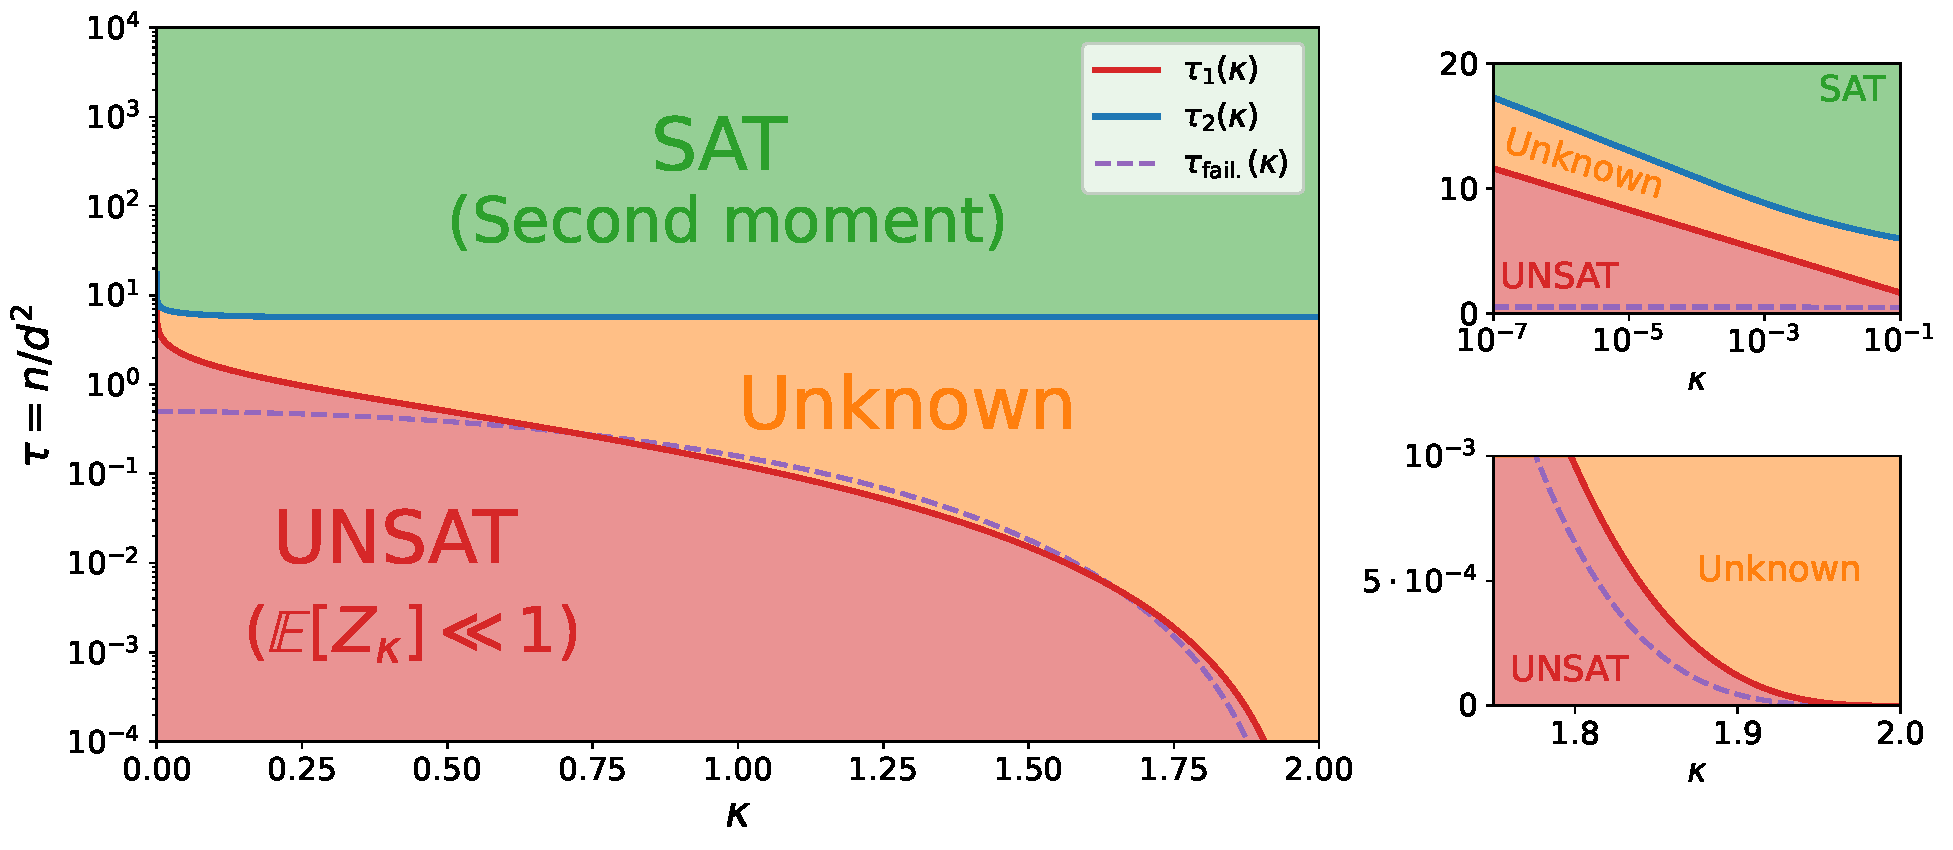
\includegraphics[width=1.0\textwidth]{figures/phase_diagram.pdf}
    \caption{
        Sketch of the satisfiable (SAT) and unsatisfiable (UNSAT) regimes in average-case matrix discrepancy, 
        as proven by Theorems~\ref{thm:first_moment} and \ref{thm:second_moment}. 
        The border of the SAT region is given by $\tau_2(\kappa)$, see Proposition~\ref{prop:tau2}. 
        Numerically, we find $\tau_2(\kappa \to 2) \simeq 5.67$.
        The orange region is not characterized by our results, and remains open.
        The dotted purple line shows $\tau_\f(\kappa)$: according to Theorem~\ref{thm:fail_second_moment}, for $\tau < \tau_\f(\kappa)$ the number of solutions 
        has large expectation and variance, and the second moment method fails (see also Fig.~\ref{fig:fail_second_moment}).
        The right plots show the limits $\kappa \downarrow 0$ (top) and $\kappa \uparrow 2$ (bottom).
        We emphasize that $\tau_1(\kappa), \tau_2(\kappa) \to +\infty$ as $\kappa \downarrow 0$.
    \label{fig:phase_diagram}}
\end{figure}
Our results characterize a large part of the $(\kappa, \tau)$ phase diagram: 
we discuss in the following some important consequences, as well as open directions stemming from our analysis.

\myskip
\textbf{Balancing $\Theta(d^2)$ random matrices -- }
An immediate consequence of Theorem~\ref{thm:second_moment} is the following corollary.
\begin{corollary}\label{cor:tau_infty}
    For any $\tau > 0$ large enough\footnotemark%
    , if $n,d \to \infty$ with $n / d^2 \to \tau$, and letting $\bW_1, \cdots, \bW_n \iid \GOE(d)$,
    then (with high probability) there exists $\eps \in \{\pm 1\}^n$ with margin 
    \begin{equation*}
        \frac{1}{\sqrt{n}} \left\|\sum_{i=1}^n \eps_i \bW_i\right\|_\op \leq \kappa_c(\tau) < 2.
    \end{equation*}
    Furthermore, $\kappa_c(\tau) \to 0$ as $\tau \to \infty$.
\end{corollary}
\footnotetext{Numerically, we find $\tau \geq 6$ is enough, see Fig.~\ref{fig:phase_diagram}.}
\noindent
Corollary~\ref{cor:tau_infty} establishes that for $n$ large enough but still in the scale $n = \Theta(d^2)$, one can find solutions 
with margin arbitrarily close to $0$.
As far as we know, our result is the first proof that a number $n = \Theta(d^2)$ of Gaussian random matrices can be balanced in a way to make 
their spectrum \emph{macroscopically shrink} compared to the typical spectrum of a Gaussian matrix: it solves an open problem posed by \cite{kunisky2023online}.


\myskip
\textbf{Tightness of the second moment analysis --}
Similarly to \cite{aubin2019storage} (and subsequent works) for the symmetric binary perceptron (SBP), we use a second moment approach to characterize the feasibility of this problem.  
However, while this method gives a tight threshold for the SBP in Theorem~\ref{thm:trans_SBP} (and thus leaves no ``Unknown'' region in the SBP counterpart to Figure~\ref{fig:phase_diagram}),
the situation in average-case matrix discrepancy is quite different.

\myskip
First, the threshold $\tau_2(\kappa)$ of eq.~\eqref{eq:def_tau2} is likely not optimal, 
as the upper bounds on $\EE[Z_\kappa^2]$ proven in Section~\ref{sec:2nd_moment} are not expected to be tight.
For this reason, the second moment ratio $\EE[Z_\kappa^2]/\EE[Z_\kappa]^2$ might still be bounded by a constant (cf.\ Proposition~\ref{prop:2nd_moment}) even for some values $\tau \leq \tau_2(\kappa)$. 
For instance, one might conjecture that this includes values of $\tau$ arbitrarily close to $0$ when $\kappa$ approaches $2$, which is not captured by our current bounds.
Improving the estimates we obtain in Section~\ref{sec:2nd_moment} to obtain a sharp study of the range of parameters $(\tau, \kappa)$ with bounded second moment ratio is significantly more complex than in the SBP setting:
it requires a precise understanding of the large deviation properties of the law of $(\|\bW_1\|_\op, \|\bW_2\|_\op)$, where $\bW_1, \bW_2$ are two correlated $\GOE(d)$ matrices, both conditioned on having small spectral norm (see eq.~\eqref{eq:def_Gd}). 
A rate function for this law can be obtained in a variational form (see e.g.\ Theorem~3.3 of \cite{guionnet2004first}), however a numerical analysis of this variational formula 
is a very challenging problem, which we leave as a future direction.

\myskip
Furthermore, and very interestingly, we show in Theorem~\ref{thm:fail_second_moment} that 
(assuming Hypothesis~\ref{hyp:control_Gsecond}) the second moment method does not yield a sharp satisfiability threshold in average-case matrix discrepancy. 
Indeed, there exists a range of $\kappa \in (0,2)$ such that 
$\tau_1(\kappa) < \tau_{c}(\kappa)$, so that if $\tau \in (\tau_1(\kappa), \tau_c(\kappa))$, 
then both $\lim (1/d^2) \log \EE[Z_\kappa] > 0$ and $\liminf (1/d^2) \log \EE[Z_\kappa^2]/\EE[Z_\kappa]^2 > 0$.
For such values of $(\tau, \kappa)$, the variance of $Z_\kappa$ is thus exponentially large (in $d^2$), and an approach based solely on the second moment method 
will fail at characterizing the feasibility of the problem.
Numerically, we find  that $\tau_1(\kappa) < \tau_c(\kappa)$ in the range $0.718 \lesssim \kappa \lesssim 1.652$. We summarize these findings in Fig.~\ref{fig:fail_second_moment}.
\begin{figure}[!t]
    \centering
    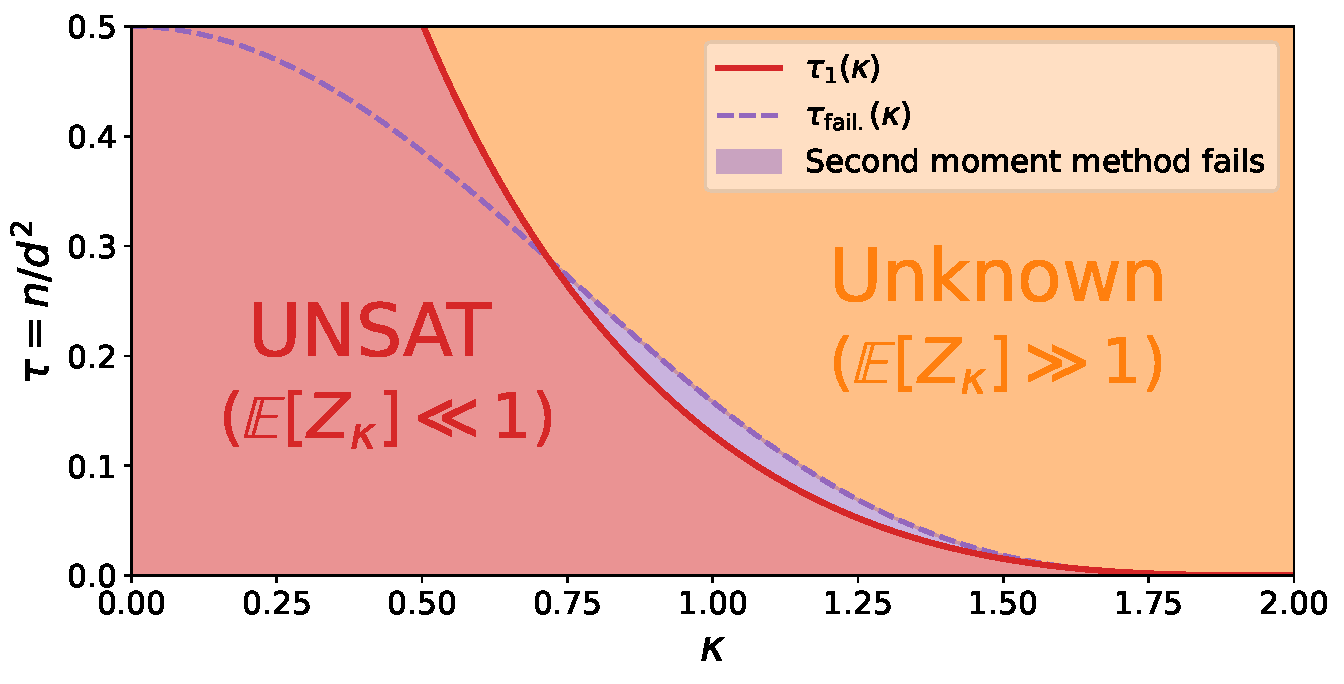
\includegraphics[width=0.75\textwidth]{figures/fail_second_moment.pdf}
    \caption{
        Illustration of Theorem~\ref{thm:fail_second_moment}. There exists a region of parameters (in purple) $\tau \in (\tau_1(\kappa), \tau_c(\kappa))$
        for which the number of solutions $Z_\kappa$ to average-case matrix discrepancy satisfies both $\EE[Z_\kappa] \gg 1$ and $\EE[Z_\kappa^2] \gg (\EE[Z_\kappa])^2$,
        so that the second moment method fails at characterizing the feasibility of the problem.
    \label{fig:fail_second_moment}}
\end{figure}

\myskip
We stress that the result of Theorem~\ref{thm:fail_second_moment} is in stark contrast with the symmetric binary perceptron, in 
which the second moment method succeeds in the entirety of the phase diagram (Theorem~\ref{thm:trans_SBP}).
In particular, this unveils a potentially richer picture for the geometry of the solution space than in the SBP.
We note that, given the proof of Theorem~\ref{thm:fail_second_moment} (see Section~\ref{sec:fail_2nd_moment}), 
we do not expect the second moment to be large because of spurious rare events, in which case one can often
still apply the second moment method by conditioning away from these rare events (see e.g.~\cite{janson1996second}, and an application in random vector discrepancy in~\cite{altschuler2022discrepancy}). 
As such, we believe that sharply characterizing the satisfiability threshold would require other techniques, that could more directly tackle the typical number of solutions 
$(1/d^2) \EE[\log Z_\kappa]$ (what is called the ``quenched'' free energy in the statistical physics jargon).
We leave such a challenging investigation for a future work.
Finally, we emphasize that the failure of the second moment method might extend to other parts of the ``Unknown'' region of the phase diagram
(beyond the purple region of Fig.~\ref{fig:fail_second_moment}) 
which are not captured by the local analysis used in Theorem~\ref{thm:fail_second_moment}: we refer to Section~\ref{sec:fail_2nd_moment} for details.

\myskip 
\textbf{Sharp threshold sequence --}
Theorem~7 of \cite{altschuler2023zero} (see also Lemma~\ref{lemma:dylan})
directly implies the existence of a sharp threshold sequence for average-case matrix discrepancy. 
Using Theorems~\ref{thm:first_moment} and \ref{thm:second_moment}, we can locate it
in the closure of the ``Unknown region'' of Fig.~\ref{fig:phase_diagram}.
\begin{corollary}[Sharp threshold sequence]\label{cor:sharp_threshold}
    \noindent
    Let $n, d \geq 1$, and assume $n/d^2 \to \tau > 0$ as $d\to \infty$. There exists a sequence 
    $\kappa_c(d,\tau)$ such that: 
    \begin{itemize}
        \item[$(i)$] For any $\eps > 0$, $\bbP[Z_{\kappa_c - \eps} \geq 1] = \smallO_d(1)$, while $\bbP[Z_{\kappa_c + \eps} \geq 1] = 1 - \smallO_d(1)$.
        \item[$(ii)$]  $\tau_1(\kappa_c) \leq \tau \leq \tau_2(\kappa_c)$, i.e.\ $(\kappa_c,\tau)$ is in the closure of the ``Unknown'' region of Fig.~\ref{fig:phase_diagram}.
    \end{itemize}
\end{corollary}
\noindent
The existence of a sharp threshold sequence has been established recently in a variety of other perceptron-like problems, see for instance \cite{talagrand1999self,talagrand2011mean,xu2021sharp,nakajima2023sharp,altschuler2023zero}.
Corollary~\ref{cor:sharp_threshold} shows the existence of a sharp threshold $\kappa_c$ depending on $d$, and bounds it in an interval of size $\Theta(1)$. 
We further conjecture $\kappa_c(d,\tau)$ to converge to a well-defined limit, as we plan to discuss in a future work.

\myskip
\textbf{Structure of the solution space --}
Beyond satisfiability, a natural question
concerns
the geometric structure 
of the space of solutions $\{\eps \in \{\pm 1\}^n \, : \, \|\sum_i \eps_i \bW_i\|_\op~\leq~\kappa \sqrt{n}\}$.
In the symmetric binary perceptron, the geometric structure of the solution space was investigated by~\cite{aubin2019storage,perkins2021frozen,abbe2022proof},
and was shown to exhibit a ``frozen-1RSB'' structure: that is, typically, solutions are isolated and far apart.
Whether the solution space in average-case matrix discrepancy presents similar geometric features is a stimulating question, especially as the failure of the second moment method in parts of the phase diagram might indicate a richer picture than in the SBP.
We leave this question open for future investigation.

\myskip 
\textbf{Algorithmic discrepancy --}
The past decade has seen a surge of interest in \emph{algorithmic discrepancy}, that is the design of efficient algorithms to produce signings 
$\eps \in \{\pm 1\}^n$ minimizing a discrepancy objective such as eq.~\eqref{eq:def_disc}. 
In the classical context of vector discrepancy, this line of work was initiated by \cite{bansal2010constructive}, and we refer to \cite{bansal2023resolving,kunisky2023online} for a more detailed description of the 
literature that followed.
For the problem of average-case matrix discrepancy, \cite{kunisky2023online} propose an online algorithm that is able to achieve a discrepancy
$\|\sum_i \eps_i \bW_i\|_\op \lesssim d \log(n+d)$ for a large class of random matrices $\bW_i$, including the $\GOE$ distribution.
In the regime $n = \Theta(d^2)$, this unfortunately falls short of obtaining a discrepancy lower than $2 \sqrt{n}$. 
Whether one can design a polynomial-time algorithm that can output (with large probability) a low-discrepancy $\eps \in \{\pm 1\}^n$ in parts of the SAT phase described in Fig.~\ref{fig:phase_diagram} 
remains an open question. 
For the symmetric binary perceptron, which is the vector analog to our problem, it was recently shown that the phase diagram presents a large computational-to-statistical gap
in which low-discrepancy solutions exist, while large classes of polynomial-time algorithms can not find them, and that this was related to the geometric structure of the solution space~\citep{bansal2020line,gamarnik2022algorithms}.
